%!TEX encoding = UTF-8 Unicode
\chapter{Aspekte}
Aspekte Aspekte
\section{Markt}
	\subsection{Markt für IT-Consulting}
	In den letzten Jahren ist der Markt für Beratungsleistungen in Deutschland stark gewachsen. Während im Jahr 1992 noch 5,9 Mrd.\texteuro Umsatz für Beratungsleistungen erzielt wurden(Quelle: BDU 2003), waren es im Jahr 2008 bereits 18,2 Mrd. \texteuro (Quelle:BDU 2009) und im Jahr 2012 betrug der Umsatz schon 22,30 Mrd. \texteuro (Abb.1).
	\begin{figure}[htp]
	\centering
	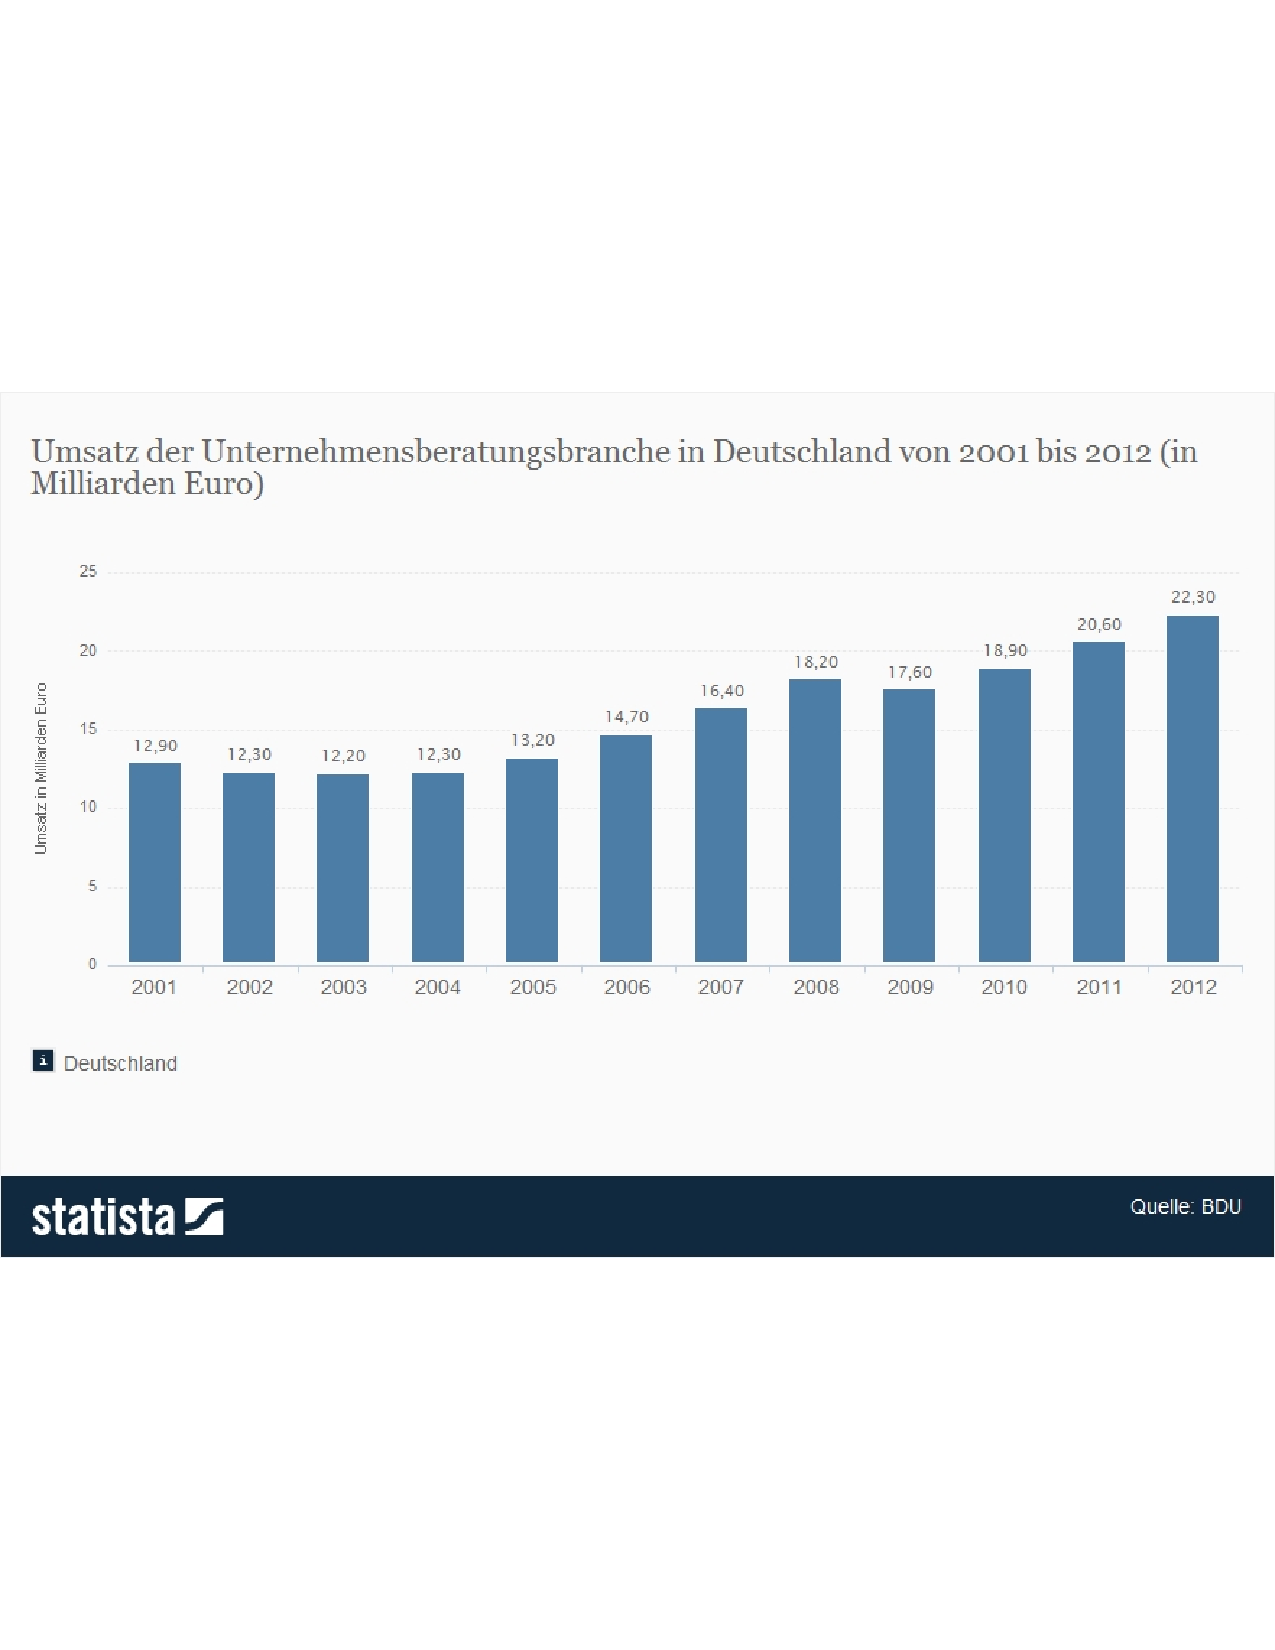
\includegraphics[width=0.5\linewidth]{./UmsatzUBeratungsbrancheDeutschland}
	\label{fig:UmsatzUBeratungsbrancheDeutschland}
	\caption{Umsatz der Unternehmen}
	\end{figure}
\section{Arbeitskultur}
	\subsection{Einleitung in das Wesen des IT-Consultings}
	
IT-Consulting ist eine wichtige Art des Consultings in IT-Fragen eines Unternehmens.Das Wesen des Consultings besteht im Großen und Ganzen darin Unternhemen bei der Neustrukturiereung des Anwendungslandschaften oder bei der Pflegung der bestehenden Informationssysteme zu unterstützen. Während des gesamten Beratungsprozesses bleibt Berater als externe Experte solange im Unternhemen bis die Probleme,die er zu lösen hat,selbständig vom Unternehmen zu lösen werden.
Um den Beratungsprozess zu verdeutlichen, wird jetzt ein Beispielprozess beschrieben. Ein Online-Handelsnternehmen möchte ein BI Standardsoftware einführen um die Daten für Analysezwecke aus dem ERP-System zu laden,um die potentiellen Kündiger zu vermeiden oder neue Kunden zu gewinnen.Am Anfang jedes Prozesses muss dem Berater die Organistationstruktur des Unternehmens klar sein, um eine passende Lösung zu finden. Im Beratungsprozess gibt es eine Standardsoftware um IT-Problem zu lösen. Es gibt aber keine Standardlösung die für alle Unternehmensstrukturen passend ist,weil die Unternehmensstrukturen sehr unterschiedlich sind. Man beginnt die Verhandlung zwischen Unternehmensführung und den Beratern, die den Auftrag bekommen, indem man Vertrag abschließt. Danach beginnt die Analysephase. Hier wird die Unternhemenstruktur des Online-Handelsunternhemen auseinadergenommen, bis man erkennt wo die Software eingesetzt wird, Stellen wo die Reibungen entstehen werden,welche Resourcen stehen zur Verfügung und welches Informationssystem sich am besten dafür eignet.
Es muss immer ein Feedbeck zwischen dem Berater und Unternehmensführer möglich sein.
nach der Analysephase beginnt die Umsetzungphase indem eine neue IT-Architektur aufgebaut wird oder die vorhandene ergäntzt wird.Im unseren Besipiel wird die ERP-lösung mit dem BI Lösung erweitert, die vorhandene Architektur bleibt erhalten. In dieser Phase können auch die andere Berater aufgerufen werden, falls es viele Realisierungsmaßnehmen gibt.
Nach dem die Informationssystem erfolgreich installiert ist beginnt die Schulungsmaßnahmen, damit die Mitarnbeiter des Unternhemen in der Lage sind mit diesem System umgehen zu können.Danach kommt die Wartungsphase.
	\subsection{Bedeutung der Arbeitskultir für IT-Consulting}
In wie weit ist es wichtig Arbeitskultur für den Beratungsprozess zu betrachten? Anhand vom unseren Beispiel ist es zu erkennen dass die Berater ständig mit den Unternehmsvertretern kommunizieren sollen.Es ist wichtig,dass die Berater genug technisches Know-how mitbringen,aber noch wichtiger sind die Soft Skills,die enntscheidend sind.´´IT Business is People's Business. Diese Leitlinie impliziert, dass der Erfolg von IT-Projekten maßgeblich von der Kompetenz des Beraters abhängt.´´
%(Quelle: http://www.it-production.com/index.php?seite=einzel_artikel_ansicht&id=26189)
 Welche Social Skills des beraters sind für Deutscher als obligatorisch herausgestuft?Sind diese persönlichen eigenschaften auch für die anderen Nationen von der Bedeutung? Beide Parteien müssen für die Lösung des Problems einig werden. Der Berater muss Unternehmen für seine vorgeschlagene Lösung überzeugen. Muss man um dies zu realisieren nur eine gute Software anbieten oder reicht es in USA nicht aus,weil der Berater ´´schwarz´´ ist. <-- Scherz xD. Für diese Arbeit ist wichtig zu wissen wie Arbeitskultur in ausgewählten Länder sich unterscheidet und in wie weit diese den Beratungsprozess beeinflüssen kann. 
Sind überhaupt Softs Skills entscheidend für einige Länder oder spielt eher die technische Ausrüstung des Beraters bedeutsame Rolle.
Schwerpunkte:\\
1)Für die Autoren dieser Arbeit ist es aus persönlichen Interessen wichtig zu wissen wie man Unternehmen aus anderen Ländern berät und indem man als Berater ins Ausland geschickt wird.\\
2)Wie verläuft der Beratungsprozess in einigen Länder die bedeutungsvoll und potenzialreich für IT-Consulting sind.

Arbeitskultur hängt stark von Kultur des betroffenden Landes(Sitten,Bräuche) ab!!!

In den folgenden Kapiteln werden Länder untersucht werden und zum Schluss einige interessante Fakten verglichen und diskutiert werden. 

\subsection{Teilaspekte der Arbeitskultur}
Hier werden Aspekte aufgelistet die für Arbeitskultur von der Bedeutung sind.(Arbeitsplatz, Mitarbeiterverhältnisse,Hierarchien,Organisation,Lebensunmstände etc.)

	\subsection{Russland}
	% was mache ich mit den Quellen in original Sprache?
	´´Russland gilt als Wachstumsmarkt mit Zukunft. Exporte und Investitionen aus Deutschland warten mit hohen Wachstumsraten auf. Die zunehmende Vernetzung mit dem ehemals weitgehend geschützten russischen Markt erfasst auch die Informationstechnologie. Dies gilt für deutsche Unternehmen, die Produktionsstätten und Akquisitionen im Osten in ihre IT-Systeme integrieren genauso wie für russische Manager, die bei der Informationstechnologie auf westliches Know-how setzen.´´\\
	%(Quelle: http://www.it-production.com/index.php?seite=einzel_artikel_ansicht&id=26189)
	
	Da der Markt noch relativ neu ist,muss man als Berater ganz viele Entscheidungen intuitiv treffen.
	Soft Skills sind gefragt!\\
	
	´´Der Zerfall der Sowjetunion und die Reformen im wirtschaftlichen und sozialen Gefüge Russlands haben einen erheblichen Einfluss auf die Arbeitskultur in gegenwärtigen russischen Organisationen.´´\\
	%Quelle http://joconsult.netzmerk.com/pup/prozess-de.pdf
		\textbf{Aspekt Arbeitsplatz}\\
	``Der Arbeitsplatz ist für viele russische Arbeitnehmer nicht nur der Ort, an dem das Einkommen erarbeitet wird, er hat auch eine große soziale Bedeutung: Familienangehörige von Kollegen kennen sich untereinander, wenn der Kindergarten geschlossen hat, bringen 
	Frauen ihre Kinder mit zur Arbeit etc. Eine Abgrenzung zwischen Berufstätigkeit und Arbeitsleben, wie sie im westeuropäischen Sinne üblich ist, wird nicht vorgenommen.``-> Wie kann die Aussage den Beratungsprozess beeinflussen?\\
	\textit{hier kommt der Text mit eigener Reflektion in Bezug auf IT-Consulting}\\
	\textbf{Aspekt Team: Russischer Arbeitskollektiv gegen westlichen Team}\\
	``Das Arbeitskollektiv wurde in der sowjetischen 
	Epoche als das zentrale soziale Handlungsfeld propagiert und die Loyalität gegenüber dem 
	Kollektiv wurde als Ausdruck der politischen Einstellung gewertet. Die Geschlossenheit 
	der Gruppe ist wichtiger als die Selbstverwirklichung des Einzelnen. Nicht selten werden 
	auch interpersonelle Konflikte und Spannung deshalb vermieden oder nicht diskutiert. 
	Damit unterscheidet sich das Kollektiv in russischen Organisationen vom Team im 
	westeuropäischen Sinne: Ein Kollektiv in russischen Organisationen ist meist eine 
	dauerhafte Einrichtung und hat klar zugewiesene Leitungskompetenzen, die vom 
	Vorgesetzten ausgeübt werden, während das Team nur für die Dauer eines bestimmten 
	Projektes eingerichtet wird und sich durch die Gleichberechtigung aller Teammitglieder 
	auszeichnet.`` 	%Quelle http://joconsult.netzmerk.com/pup/prozess-de.pdf
	\textit{hier kommt der Text mit eigener Reflektion in Bezug auf IT-Consulting}
	\\
	\textbf{Aspekt Organisation}\\
	Russische Organisationen zeichnen sich durch eine Konzentration von Macht auf die 
	Führungskräfte aus. Ohne den “Natschalnik” werden keine Entscheidungen getroffen. 
	Führung in russischen Organisationen setzt einen starken Akzent auf die Kontrolle (im 
	Sinne von Überwachung). Die Förderung und Beratung von Mitarbeitern im Sinne eines 
	Zugewinns von Fähigkeiten und Wissen ist in Russland nicht sehr verbreitet. Hier scheint 
	Führung auf Aufsicht begrenzt zu sein. Eine Verlagerung von Entscheidungskompetenz 
	auf unterstellte Mitarbeiter wird kaum praktiziert. 
	Seitens der unterstellten Mitarbeiter werden Entscheidungen der Führungskräfte oft 
	widerspruchslos akzeptiert. Es herrscht die Einstellung vor: “Der Chef muss es ja wissen”. Entscheidungen werden häufig ausgeführt, auch wenn die dahinter stehenden Fakten 
	unbekannt sind oder die Entscheidung nicht für richtig befunden wird. Eine aktive 
	Auseinandersetzung zwischen Vorgesetzen und Mitarbeitern über den “richtigen” und in 
	diesem Fall gemeinsamen Weg ist sehr selten. Damit tragen Vorgesetze die alleinige 
	Verantwortung - Mitarbeiter führen lediglich Anweisungen aus. Das Vertrauen in die 
	Lernfähigkeit und damit in den Zugewinn von Kompetenz der Mitarbeitern seitens der 
	Vorgesetzten ist gering. 
	\textit{hier kommt der Text mit eigener Reflektion in Bezug auf IT-Consulting}
	 

	\subsection{China}
	
	
	\subsection{USA}
	
	
	\subsection{Deutschland}
	
	
	\subsection{Indien}


\section{Wissenschaft}